\documentclass{standalone}
\usepackage{tikz}
\usepackage{dsfont}
\usepackage{amsmath, amsthm, amssymb}
\usetikzlibrary{matrix}
\newcommand*\Z{\mathds{Z}}
\newcommand*\CP{\mathbb{CP}}
\newcommand*\ee[2]{H^{#1}(\CP^2) \otimes_{\Z} H^{#2}(S^1)}
\newcommand*\zt[2]{#1 \otimes_{\Z} #2}
\newcommand*\HT[2]{H^{#1}(\CP^2) \otimes_{\Z} #2}
\newcommand*\HCP[1]{H^{#1}(\CP^2)}
\begin{document}
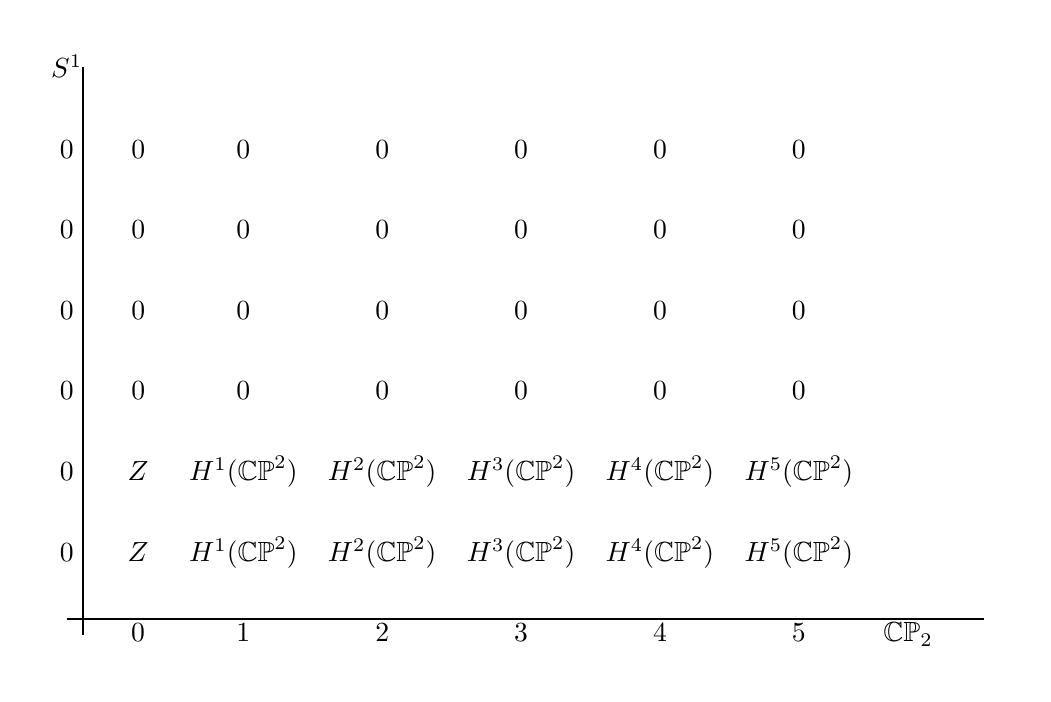
\begin{tikzpicture}
\matrix (m) [matrix of math nodes,
  nodes in empty cells,nodes={minimum width=5ex,
  minimum height=5ex,outer sep=-5pt},
  column sep=1ex,row sep=1ex]{
%
S^1&    &   &   &   &   &   &   &   \\
%
0&  0&      0&  0&  0&  0&  0&  &\\
0&  0&      0&  0&  0&  0&  0&  &\\
0&  0&      0&  0&  0&  0&  0&  &\\
0&  0&      0&  0&  0&  0&  0&  &\\
0&  \Z& \HCP{1}&    \HCP{2}&    \HCP{3}&    \HCP{4}&    \HCP{5}&    &\\
0&  \Z& \HCP{1}&    \HCP{2}&    \HCP{3}&    \HCP{4}&    \HCP{5}&    &\\ \quad\strut
%
&   0&  1&  2&  3&  4&  5&  \CP_2& \strut \\};
%
\draw[thick] (m-8-1.east) -- (m-1-1.east) ;
\draw[thick] (m-8-1.north) -- (m-8-9.north) ;
\end{tikzpicture}
\end{document}